\scanpage{49}
\mspage{5)}
Cette opération de sommes est la plus triviale parmi les opérations qu'il
nous faudra expliciter et transcrire (combinatoirement) dans la suite.
Notons de suite, pour $(X,\widetilde\Sigma,R)$ donné
\[
X\deleted{\unsure{\Sigma}}\text{ connexe}\Longleftrightarrow
\Gamma\mathrm{MD}(X,\widetilde\Sigma,R)\text{ connexe}
\]
plus précisément
\[
\pi_0(X)\simeq\pi_0(\Gamma\mathrm{MD}(X,\widetilde\Sigma,R))
\]
\margin{donner la formule pour le genre d'un
$\alpha\in\pi_0(X)\simeq\pi_0(\Gamma)$ en termes de la pondération ---
plus généralement \unsure{donner} le \uline{genre total} est
\[
g=\sum_{s\in S}g_s+c(\Gamma)
\]
\unsure{indice de connexion} du graphe
$=\deleted{\unsure{\chi}}\unsure{\mathrm{rg}\,H^1(\Gamma)}$.}

\uline{Cas particuliers.}

a) Cas de $S_*\mathcal T^\pm_{\mathrm{top}}\
\deleted{\unsure{S_*\mathcal T_{\mathrm{top}}}}$
--- i.e. $\Sigma=\varnothing$, $\widetilde\Sigma=\partial X$.

Cela correspond au cas des graphes MD \deleted{que} où
\inserted{toutes les arêtes sont libres, i.e.}
tous les sommets sont isolés (sauf arêtes libres)
\deleted{Il} \inserted{Le graphe} est donc déterminé par
\diagram{\begin{tikzcd}[ampersand replacement=\&,column sep=large]
A\ (\simeq\vec A=\vec A^\sigma)\arrow[r,"\unsure{r|\rho}"]\arrow[d]\&\mathbb N\\
S\arrow[r,"\gamma"]\&\mathbb N
\end{tikzcd}}

Le cas de $\mathcal T^\pm_{\mathrm{top}}$ correspond à faire $\rho=0$,
donc la situation est donnée par
\diagram{\begin{tikzcd}[ampersand replacement=\&]
A=\unsure{A_0|A_\ell}\arrow[d]\&\\
S\arrow[r,"\gamma"]\&\mathbb N.
\end{tikzcd}}

\margin{\figure{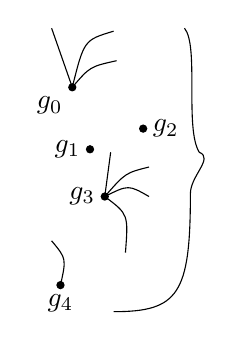
\begin{tikzpicture}[scale=.75]
\fill(0,0)circle(2pt);\node[below left]at(0,0){$g_0$};
\draw(0,0)--(-.35,1) (0,0)..controls(.2,.8)..(.7,.95)
(0,0)..controls(.3,.35)..(.75,.45);
\fill(.3,-1.05)circle(2pt);\node[left]at(.3,-1.05){$g_1$};
\fill(1.2,-.7)circle(2pt);\node[right]at(1.2,-.7){$g_2$};
\fill(.55,-1.85)circle(2pt);\node[left]at(.55,-1.85){$g_3$};
\draw(.55,-1.85)--(.65,-1.1)
(.55,-1.85)..controls(.9,-1.45)..(1.3,-1.35)
(.55,-1.85)..controls(.95,-1.65)..(1.3,-1.85)
(.55,-1.85)..controls(.95,-2.15)..(.9,-2.8);
\fill(-.2,-3.35)circle(2pt);\node[below]at(-.2,-3.35){$g_4$};
\draw(-.2,-3.35)..controls(-.1,-2.9)..(-.35,-2.6);
\draw(1.9,1)..controls(2.15,.7)and(1.9,-.7)..(2.15,-1.1)
..controls(2.4,-1.2)and(2,-1.5)..(2,-1.8)
..controls(2,-3.5)and(1.8,-3.8)..(.7,-3.8);
\end{tikzpicture}}}

Le cas d'une \uline{structure} connexe
$(\mathrm{card.}\,S=1\inserted{\text{ i.e. }S=\{s\}})$
\deleted{type $(g,\nu)$ d'une}
est \deleted{\unsure{homéomorphisme}}\inserted{caractérisé}
par la donnée des deux entiers $(g,\nu)$
$(g=\text{genre},\ \nu=\text{nb de trous})$
\[
g=\gamma(s),\qquad \nu=\mathrm{Card}\,A.
\]
\mspage{48}
